%%%%%%%%%%%%%%%%%%%%%%%%%%%%%%%%%%%%%%%%%%%%%%%%%%%%%
%			HLAVIČKA								%
%%%%%%%%%%%%%%%%%%%%%%%%%%%%%%%%%%%%%%%%%%%%%%%%%%%%%
\documentclass[openany,12pt]{memoir}

\usepackage[utf8]{inputenc} 
\usepackage[czech]{babel}
\usepackage[T1]{fontenc}
\usepackage[top=1.5cm, bottom=2cm, left=2cm, right=2cm]{geometry}  % --> NASTAVENÍ OKRAJŮ
\usepackage{fancyhdr}
\usepackage{graphicx}
\usepackage{lmodern}
\usepackage{xwatermark}
\usepackage{xcolor}
\usepackage{changepage}




%%%%%% Package na zpěvník
\usepackage[full]{leadsheets}%http://mirrors.nic.cz/tex-archive/macros/latex/contrib/leadsheets/leadsheets_en.pdf   --> dokumentace	
\definesongtitletemplate{empty}{} 
\setchords{
format = \bfseries,   %tučné akordy
minor = {mi},% 
input-notation = {german},%
output-notation = {german}%
}
\definesongtitletemplate{empty}{} 

\newlength{\drop}
\newwatermark[allpages,color=red!50,angle=0,scale=2, xpos=0,ypos=0]{
\includegraphics[width=5cm]{obr/pozadi.jpg}} %--> dvojka na pozadí


%%%% Vlastní příkazy
\newcounter{Slokočet}   %Automatické číslování slok
\newcommand{\mezera}{\vspace*{0.5cm}}   %Horizontální odsazení slok
\newcommand{\stred}{5.2cm}   %%% Na zarovnání slok doprostřed, pozn. automatičtější zarovnávání na střed nejde
\newcommand{\refren}{\mezera \noindent \textbf{R:} } %refrén
\newcommand{\sloka}{\mezera \noindent \addtocounter{Slokočet}{1} \arabic{Slokočet}. } 	%sloka, která se automaticky čísluje
\newcommand{\ssloka}{\mezera \noindent}  % vlastní číslo sloky


%%%%%%%%%%%%%%%%%%%%%%%%%%%%%%%%%%%%%%%%%%%%%%%%%%%%%%
%			NÁVOD									 %
%%%%%%%%%%%%%%%%%%%%%%%%%%%%%%%%%%%%%%%%%%%%%%%%%%%%%%
%1. Věci v hlavičce IGNOROVAT
%2. Píseň psát do prostoru mezi \begin{song} a \end{song}
%3. další řádek se značí dvěma odsazeníma (= dvakrát stisknout enter)
%4. \refren vždy na začátku refrenu a \sloka na začátek sloky (automaticky se čísluje)
%  \ = alt gr + q ; [/] = alt gr f/g ; {/} = alt gr + b/n; ^ = alt gr + 3 + mezera
%Cokoliv napíšete do ^{  } se bude brát jako akord
%když se toto bude dotýkat nějakého slova (nebude mezi tím a slovem mezera)
%tak se akordy zjeví nad slovem, ale pište to před slovo
%Když se to nedotýká slova, tak akord lítá ve vzduchu a vytiskne se větší mezera
%První možnost je asi preferovanější
%5. Akordy stačí psát jen do první sloky, když se nezmění -- kytaristi to zvládnou



%<++>
%\usepackage{subfiles}
%</++>

\begin{document}

\pagestyle{empty}
%\addtocontents{toc}{\protect\thispagestyle{empty}}
%\tableofcontents \thispagestyle{empty}\newpage
\newgeometry{top=1.5cm, bottom = 0cm, left = 2cm, right = 2cm}



\begin{song}{title=\centering Kluziště \\\normalsize Karel Plíhal \vspace*{-0.3cm}}  %% sem se napíše jméno songu a autor
\moveright 4cm \vbox{      %Varianta č. 1  ---> Jeden sloupec zarovnaný na střed	

\sloka 
	^{C{\color{white}aaaa}}Strejček ^{Emi7/H}kovář ^{Ami7}chytil ^{C/G}kleště, 

	^{Fmaj7}uštíp' z ^{C}noční ^{\,\,\,Fmaj7\,\,G}oblohy
	
	jednu malou kapku deště, ta mu spadla pod nohy.
	
	Nejdřív ale chytil slinu, tak šáh' kamsi pro pivo,
	
	pak přitáhl kovadlinu a obrovský kladivo.

\refren
	Zatím ^{C}tři bílé ^{Emi7/H}vrány ^{Ami7}pěkně za ^{C/G}sebou
	
	kolem ^{Fmaj7}jdou, někam ^{C}jdou, do ^{D7}rytmu se ^{G}kývají,

	tyhle ^{C}tři bílé ^{Emi7/H}vrány ^{Ami7}pěkně za ^{C/G}sebou
	
	kolem ^{Fmaj7}jdou, někam ^{C}jdou, ^{Fmaj7}nedojdou, ^{C}nedojdou.


\sloka	
	Vydal z hrdla mocný pokřik ztichlým letním večerem,
	
	pak tu kapku všude rozstřík' jedním mocným úderem.
	
	Celej svět byl náhle v kapce a vysoko nad námi.
	
	Na obrovské mucholapce visí nebe s hvězdami.

\refren

\sloka
	Zpod víček mi vytrysk' pramen na zmačkané polštáře,
	
	kdosi mě vzal kolem ramen a políbil na tváře,
	
	kdesi v dálce rozmazaně strejda kovář odchází,
	
	do kalhot si čistí dlaně umazané od sazí. 


}
\setcounter{Slokočet}{0}

\begin{center}
	\vspace*{1.0in}
	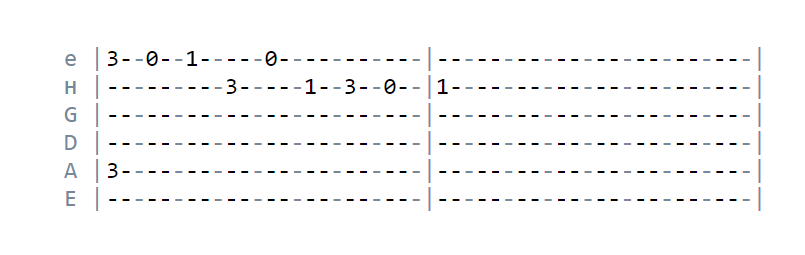
\includegraphics[scale=0.5]{../taby/kluziste.PNG}

\end{center}

	
\end{song}


\newpage


\end{document}
